\chapter{Method}
\label{cap:Method}
This chapter covers the method used in this research, including choices made in the smart home architecture, capturing, filtering and analysis processes. Further the logical structure of the detection algorithms are presented. The entire method is broken down into several stages to better structure the research, as illustrated in Figure \ref{fig:Method_process}.  

\begin{figure}[H]
    \centering
    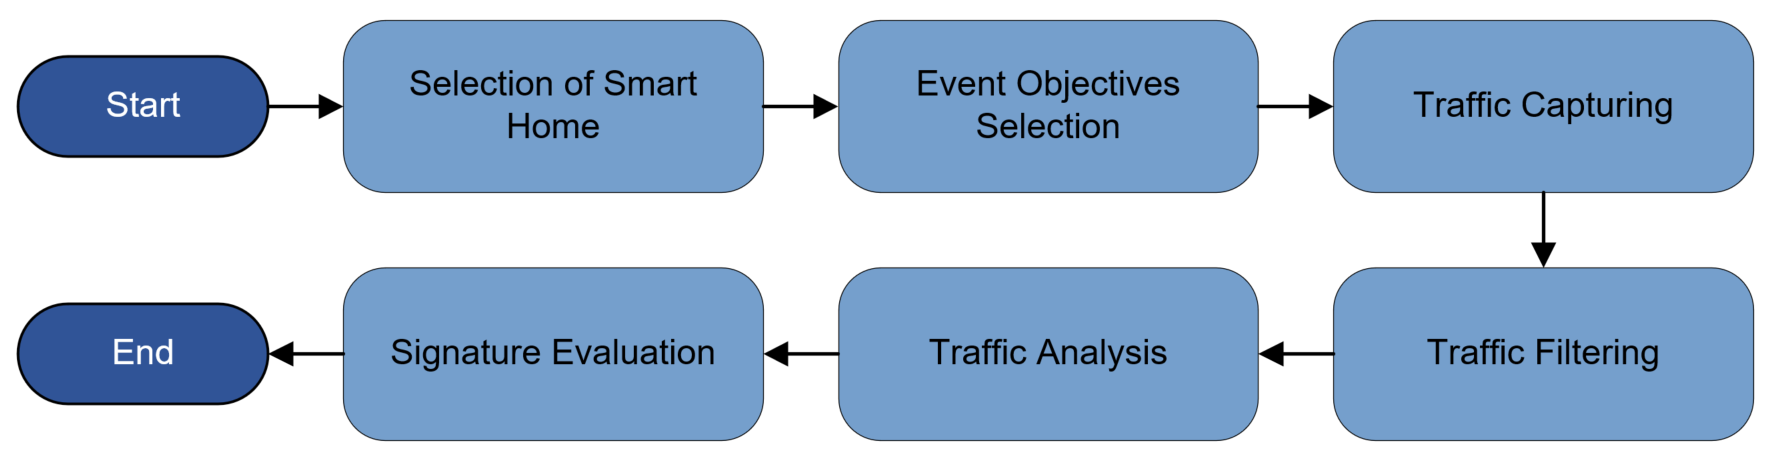
\includegraphics[width=\textwidth]{figures/Method_process.png}
    \caption{Overview of the stages within the thesis structure}
    \label{fig:Method_process}
\end{figure}



\section{Selection of Smart Environment}
This research used only one robot vacuum cleaner which was selected based on a set of requirements, a survey was therefore conducted at the start of the research. A selection process for the associated smart home environments was also conducted trying to simulate a general smart home.

Requirements within three different categories were used to select the device: \textit{communication protocols, smart home features} and \textit{popularity} were used in the selection process. These requirements are described below:  

\begin{itemize}
    \item Communication protocol: Wi-Fi is the most wide spread communication protocol in today's smart environments \cite{robotsel1}. Eavesdropping devices and analysis tools are available for IEEE.802.11 and abstraction layers higher in the OSI model \cite{osimodel}. Therefore the first requirement for the RVC will be that it communicates over Wi-Fi.
    
    \item Smart Home Features:  The number features available, could increase attribution and potentially more information could be exposed. The robot vacuum cleaner needs to have several smart home features to test \cite{robotsel4}.
    
    \item Popularity: The prevalence of different vendors and models will always vary, based on the number of sold and used devices. Overall usage and good reviews will increase the relevance and the scientific contribution of this thesis. Therefore popularity is included in the evaluation of RVC.
\end{itemize}

Data and ratings from three robot vacuum cleaner review sites \cite{robotsel11}, \cite{robotsel12} and \cite{robotsel13} were used in the first phase of the selection. A summary of all these reviews was used to determine the most reliable robot vacuum cleaner vendors. To determine the popularity of the different vendors, downloadings and ratings from Google Play were compared \cite{GooglePlay}.

Results from the review sites are presented in Table \ref{tab:Robotreviewsites}, and shows that the two best rated robot vacuum cleaner vendors are Irobot and Roborock.
\begin{table}[H]
    \centering
    \caption{Robot vacuum selection review-site comparison}
    \begin{subtable}[b]{0.45\linewidth}
        \centering
        \caption{Results from review-site \cite{robotsel11}}
        \begin{tabular}{|c|c|}
            \hline 
            \textbf{Vendor} & \textbf{Number on top ten} \\ \hline
            Irobot      & 3                 \\                   \hline
            Roborock    & 3                 \\                   \hline
            Neatsvor    & 0                 \\                   \hline
            Ecovacs     & 0                 \\                   \hline
            iLife       & 2                 \\                   \hline
        \end{tabular}
    \end{subtable}
    \hspace{0.5cm}
    \begin{subtable}[b]{0.45\linewidth}
        \centering
        \caption{Results from review-site \cite{robotsel12}}
        \begin{tabular}{|c|c|}
            \hline
            \textbf{Vendor}    & \textbf{Number on top ten} \\ \hline
            Irobot      & 2                 \\                   \hline
            Roborock    & 2                 \\                   \hline
            Neatsvor    & 0                 \\                   \hline
            Ecovacs     & 2                 \\                   \hline
            iLife       & 1                 \\                   \hline
        \end{tabular}
    \end{subtable}
    \begin{subtable}[b]{0.45\linewidth}
        \centering
        \caption{Results from review-site \cite{robotsel13}}
        \begin{tabular}{|c|c|}
            \hline
            \textbf{Vendor}    & \textbf{Number on top ten} \\ \hline
            Irobot      & 2                 \\                   \hline
            Roborock    & 2                 \\                   \hline
            Neatsvor    & 3                 \\                   \hline
            Ecovacs     & 1                 \\                   \hline
            iLife       & 0                 \\                   \hline
        \end{tabular}
    \end{subtable}
    \hspace{0.5cm}
    \begin{subtable}[b]{0.45\linewidth}
        \centering
        \caption{Summary of all review-sites}
        \begin{tabular}{|c|c|}
            \hline
            \textbf{Vendor}    & \textbf{Number on top ten} \\ \hline
            Irobot      & 7                 \\                   \hline
            Roborock    & 7                 \\                   \hline
            Neatsvor    & 3                 \\                   \hline
            Ecovacs     & 3                 \\                   \hline
            iLife       & 3                 \\                   \hline
        \end{tabular}
    \end{subtable}
    \label{tab:Robotreviewsites}
\end{table}

Applications for different vendors' robot vacuum cleaners are presented in Table \ref{tab:VendorApplicationStat}. It is worth mentioning that the "Smart Life" application is used to control the Neatsvor vacuum cleaner, but is primarily a smart home integration application. 

\begin{table}[H]
\centering
\caption{Robot vacuum cleaner applications download and rating statistics}
\label{tab:VendorApplicationStat}
\begin{tabular}{|c|c|c|c|}
\hline
\textbf{Vendor} & \textbf{Application} & \textbf{Downloads} & \textbf{Rating} \\ \hline
Irobot          & Irobot Home          & 5 million +        & 4,0/5,0         \\ \hline
Roborock        & Roborock             & 1 million +        & 4,6/5,0         \\ \hline
Neatsvor        & Smart Life           & 10 million +       & 4,5/5,0         \\ \hline
Ecovacs         & Ecovacs Home         & 1 million +        & 2,5/5,0         \\ \hline
iLife           & iLifehome            & 50 thousand +      & NA              \\ \hline
\end{tabular}
\end{table}
Both Irobot and Roborock received seven recommendations on the review websites combined. This is significantly higher than the other three vendors on the list, each of which only had three representations. Additionally, both vendors were referenced in all three review sites which strengthens their credibility. 

In the application download and rating analysis, the Neatsvor application has over 10 million downloads. However, this application is more focused on smart home integration, and the high number of downloads is likely not solely due to the robot vacuum cleaner. Meanwhile, Ecovacs home received a 2.5/5.0 rating, and despite having a similar number of downloads as Roborock, it fell short in the selection process. Hence, Irobot and Roborock emerged as the two most relevant vendors. In a comparison of their products, it was found that the Irobot Roomba i7 and Roborock S6 were the most suitable, they include a wide range of smart home features, uses Wi-Fi as their main communication protocol and are the most popular \cite{robotsel8} \cite{robotsel6}. 

The final comparison was conducted using \textit{bestcordlessvacuumsite.com} \cite{robotsel9}. Irobot Roomba i7 and Roborock S6 have similar reviews and rating all over, and they both have a sufficient number of smart home features, such as IoT smart home integration, application, different cleaning types and detailed environment discovery. The fact that the Irobot application is downloaded 5 times more than the Roborock was the decisive factor. Irobot Roomba i7 is the selected robot vacuum cleaner for this master project and is presented in Figure \ref{fig:irobotroombai7}. 

\begin{figure}[H]
    \centering
    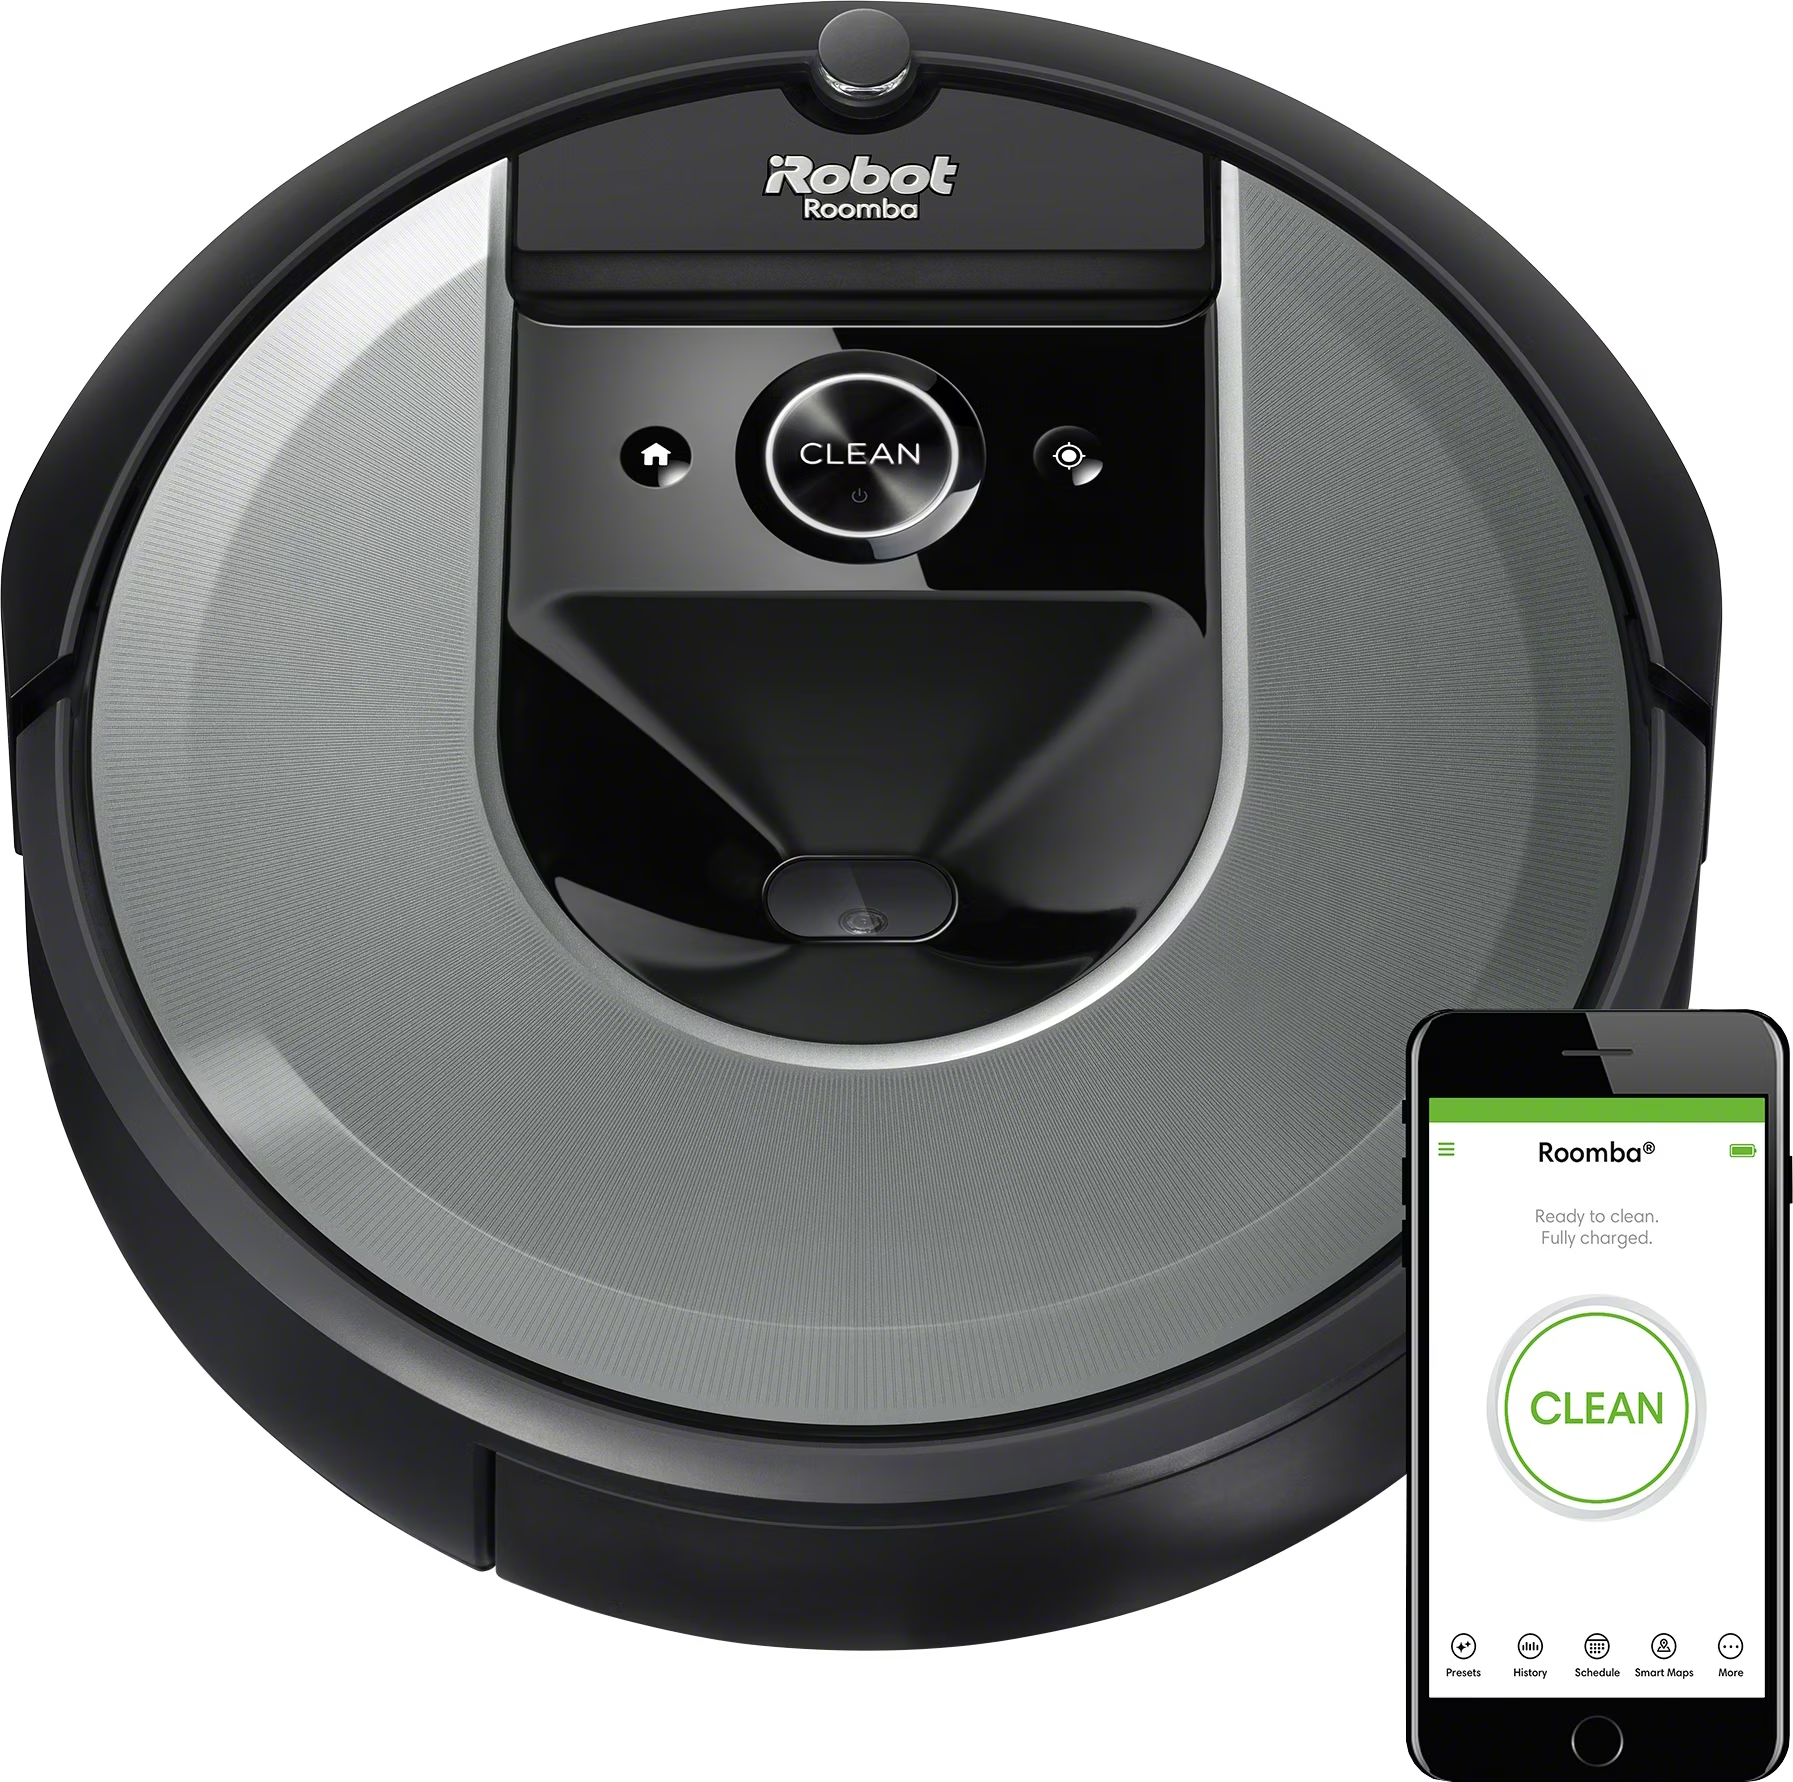
\includegraphics[width=0.5\textwidth]{figures/Irobot_picture.png}
    \caption{Irobot Roomba i7 \cite{irobotroombai7_picture}}
    \label{fig:irobotroombai7}
\end{figure}

To ensure the validity of the results across diverse settings, the testing was conducted in two different smart environments, now called \textbf{Oslo} and \textbf{Drammen}. The robot vacuum cleaner was configured from factory defaults for each of the environment. Both \textbf{Oslo} and \textbf{Drammen} had independent Internet access, provided by an external Internet Service Provider (ISP). To control the duration of each test, the available test area was restricted to one room. This decreased the duration of each test, making the research more efficient. Illustrations of both \textbf{Oslo} and \textbf{Drammen} smart environments are presented in Figure \ref{fig:SmartHomeEnvironments}.

\begin{figure}[H]
    \centering
    \begin{subfigure}[b]{0.60\textwidth}
        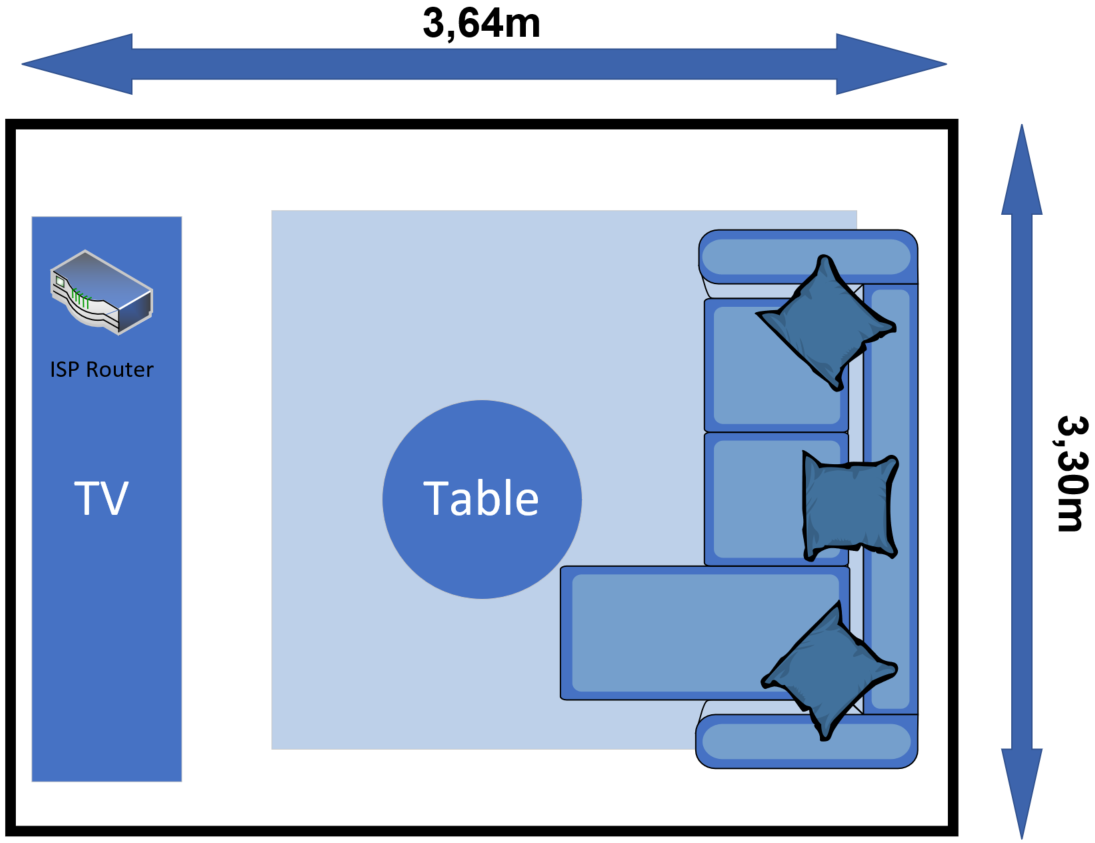
\includegraphics[width=\textwidth]{figures/Environment1.png}
        \caption{Oslo smart home environment}
        \label{fig:Environment1}
    \end{subfigure}
    \hfill
    \begin{subfigure}[b]{0.75\textwidth}
        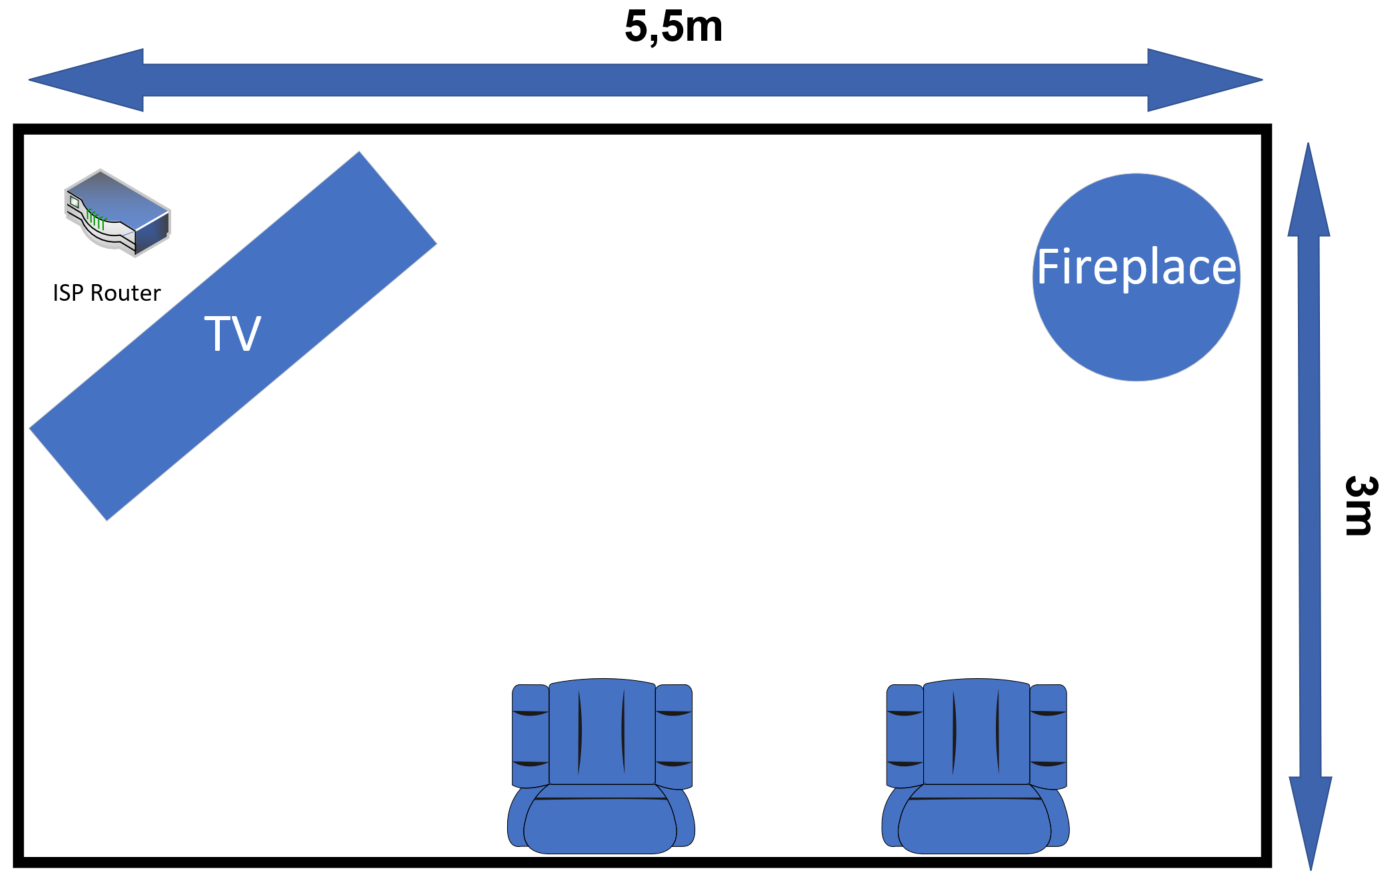
\includegraphics[width=\textwidth]{figures/Environment2.png}
        \caption{Drammen smart home environment}
        \label{fig:Environmet2}
    \end{subfigure}
    \caption{The physical configuration of the smart home environment in Oslo and Drammen}
    \label{fig:SmartHomeEnvironments}
\end{figure}

The rest of the research environment had to support traffic eavesdropping and analysis of the Irobot Roomba i7. This sets some requirements for the selection of smart environment. It has to include an AP providing a separate SSID only to be used by the Irobot Roomba i7. This way the identification of relevant and irrelevant traffic is possible without interference by other connected IoT devices. In addition to this, a wired network infrastructure needs to be available providing LAN access to the traffic generated from the Irobot Roomba, this is where the LAN eavesdropping is conducted. Lastly the environment would need Internet connectivity to be able to connect to Irobot cloud services and be controlled by a smart home application. 

A Raspberry PI 3b+ was chosen as the capturing platform for this research. These computers are designed to run autonomously and has build in Ethernet and WiFi NICs. The Raspberry PI was installed with a Kali Linux operating system from \cite{kalidownload}. Several network traffic analysis and capturing tools are included in the Kali Linux distribution. During wireless capturing, the wireless NIC had to be configured in \textit{monitor mode}. A separate Wi-Fi adapter \textit{TP-LINK TL-WN722N V2/V3} was acquired and used as the monitoring wireless NIC.

Both \textbf{Oslo} and \textbf{Drammen} only had a single ISP modem, providing both WLAN and LAN. To enable WAN interface simulation and eavesdropping, an additional Access Point (AP) and LAN switch were installed. The AP translated all Wi-Fi traffic generated form the Irobot Roomba with Network Address Translating (NAT) to a single IP address in the smart environment LAN, simulating a WAN interface. The AP then forwarded traffic to the ISP router through the switch. All traffic forwarded on the interface connected to the AP were duplicated and forwarded to the Raspberry PI, on the configured SPAN port. The network infrastructure is shown in Figure \ref{fig:WLAN_LAN_setup}, where the monitored and SPAN configured interfaces show how the eavesdropping is carried out. 

\begin{figure}[H]
    \centering
    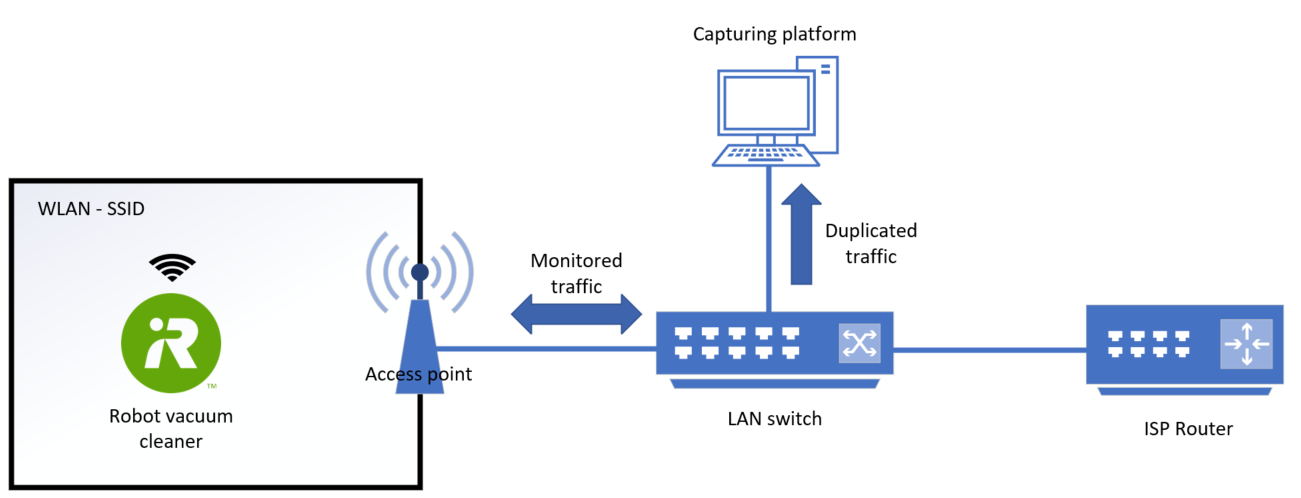
\includegraphics[width=\textwidth]{figures/WLAN_LAN_setup.png}
    \caption{WAN simulating and eavesdropping in the smart environment}
    \label{fig:WLAN_LAN_setup}
\end{figure}


Wireshark \cite{wireshark} is a widely used network protocol analyser which allows network capturing and analysis in real-time. It can be used for deep header inspection in all network layers and perform basic identification of a wide range of different protocols \cite{wireshark}. This software is integrated on Kali Linux OS and is available for Windows at \cite{wireshark_download_2016}. Tshark is a subprocess of Wireshark, and can be used to capture traffic through CLI. In this process it is possible to define capturing filters which only store traffic that is interesting for the analysis phase. Tshark was therefore used to capture traffic, and the manual analysis was done with Wireshark.

The network infrastructure in both environments consists of the devices presented in Table \ref{tab:networkdevices} and are connected in a smart environment infrastructure shown in Figure \ref{fig:SmartHomeSetup}. Telia was the ISP in both \textbf{Oslo} and \textbf{Drammen} and the same Sagemcom router was used, this did not affect the internal Irobot Roomba communication since the only function of Sagemcom is DHCP and Internet connectivity. 

\begin{table}[H]
\centering
\caption{Smart environment device inventory}
\label{tab:networkdevices}
\begin{tabular}{|c|c|}
\hline
\textbf{Device}    & \textbf{Type}                      \\ \hline
Capturing platform & Raspberry PI 3b+, with Kali Linux  \\ \hline
Analysis platform  & HP Elitebook, with Windows 11      \\ \hline
Access point       & TP-Link archer MR200, ver5.30      \\ \hline
LAN switch         & Cisco catalyst 2960 series, 8 port \\ \hline
ISP router         & Sagemcom, Telia                    \\ \hline
\end{tabular}
\end{table}



\begin{figure}[H]
    \centering
    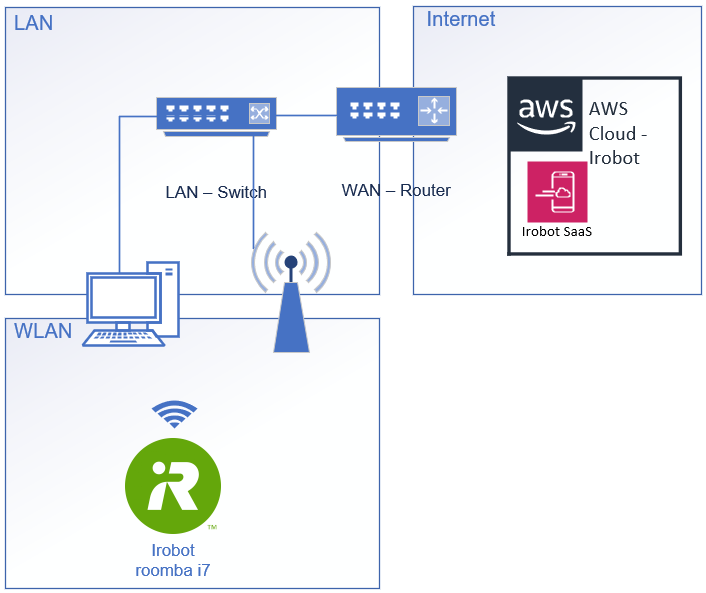
\includegraphics[width=0.8\textwidth]{figures/SmartHomeSetup.png}
    \caption{Smart home setup}
    \label{fig:SmartHomeSetup}
\end{figure}

\section{Traffic Capturing} 

Two Tshark processes were executed simultaneously on the Raspberry PI, one instance captured WAN traffic on the Ethernet NIC (eth0) and the other captured WLAN traffic on the Wi-Fi adapter NIC (wlan1). Both instances had a capturing filter argument, capturing only traffic relevant for the analysis phase. The syntax for the Tshark filter is described in \cite{tshark_filter}. The Tshark arguments used in these captures were interface specification \textit{-i}, traffic filter \textit{-f} and output file name \textit{-w}. Filtering was based on the Irobot Roomba's Wi-Fi MAC address for WLAN, and the simulated WAN IP-address for LAN. Due to local user restrictions, the Tshark commands were executed in sudo mode. Tshark filter syntax as well as WLAN and LAN specific syntax are listed below. 

\begin{itemize}
    \item tshark [ -i <capture interface> ] [ -f <capture filter> ] [ -w <outfile> ]
    \item sudo tshark -i wlan1 -f 'eth.host MAC address' -w output.pcap
    \item sudo tshark -i eth0 -f 'ip.host WAN address' -w output.pcap
\end{itemize}

A fixed capturing process was used the entire research, this created the best foundation for event comparison. The entire capturing process is illustrated in a flow diagram in Figure \ref{fig:captuingprocess}. First both WLAN and LAN Tshark capturing were started. While these captures were ongoing, events were triggered according to a test matrix. When all events had been triggered, the capturing was stopped and files were extracted with WinSCP to a Windows machine for further analysis \cite{winscp2023}.
  
\begin{figure}[H]
    \centering
    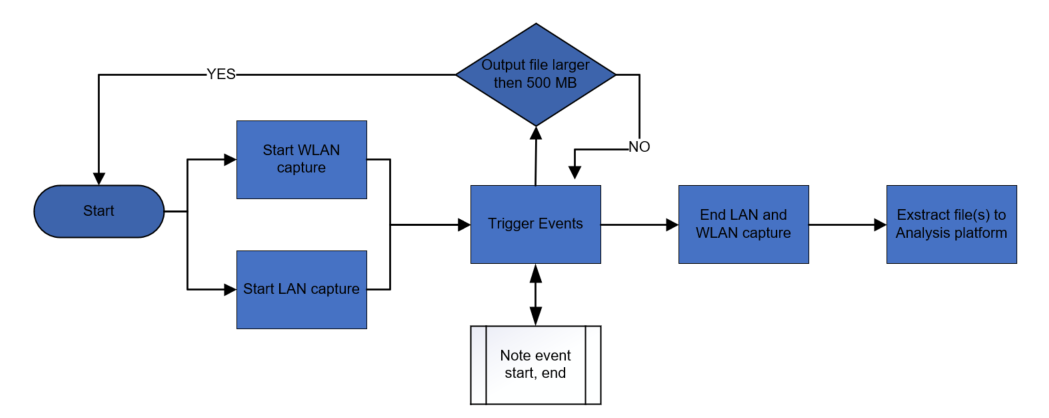
\includegraphics[width=\textwidth]{figures/Event triggering process.png}
    \caption{Capturing process}
    \label{fig:captuingprocess}
\end{figure}

\section{Event Objectives}

This section introduces the selection and triggering of different smart home features on the Irobot Roomba i7. For all selected event objectives the justification, functionality and triggering process are described. All event objectives, except \textit{Standby traffic}, are triggered 10 times in each of the smart environments \textbf{Oslo} and \textbf{Drammen}.

\textit{Standby traffic} capture is an event selected and is providing information about the continuous traffic flow generated by the Irobot Roomba when no event is triggered. This event is therefore used to identify network traffic which is not relevant in the event detection process and can be excluded for event analysis. Identified traffic is also used to identify the ongoing network session between the Irobot Roomba and the cloud server and exclude traffic generated from other IoT devices within the same environment. If an attacker can identify the present of an Irobot Roomba it can launch targeted attack such as spare phishing and increase the success rate. 

The capturing started after the Irobot Roomba had been operational in \textbf{Oslo} smart environment for one month, ensuring that the captured traffic is generated when the vacuum cleaner is in operating state and not set-up phase. A continuous capture was conducted over 14 days. During this time no physical or application interaction was done by the user. The capture was then extracted to the analysis platform.

All other event objectives aims to expose different user behaviours and each of them are described further in detail. \textit{Automated cleaning}, is a cleaning event triggered by integration with third party IoT systems. Through the Irobot application it is possible to configure integration with IFTTT location services \cite{ifttt}, triggering a cleaning when the users phone is observed outside a configured radius of the smart environment. It is also possible to integrate with Gust smart lock system, Ecobee thermostat system, My Leviton smart home integration and MyQ garage system \cite{irobot}. IFTTT was selected as the preferred trigger integration due to the availability. If this event is attributed an attacker will know when the user has left the smart environment and can potentially conduct robbery without the risk of the user being home or map the users routines such as working hours.

The location service is configured to trigger a cleaning event including the entire smart home map when the user's phone is more then 200 meters away from the address of the smart environment. Event start is defined at the time when a notification was received stating that cleaning is triggered, and finished when a "finished cleaning" notification is received. \textit{Automated cleaning} events are only triggered once per day, but due to time constrains the configured cleaning job was deleted and reconfigured for each event, allowing the event to be triggered several times per day.  

\textit{Application triggered cleaning}, is triggered through the Irobot smart phone application. Users can configure customized cleaning events only including parts of the smart environment.The event is triggered by opening the Irobot application and manually triggering a customized cleaning event defining all of the smart environment area. It is started when the application is opened and finished when the "finished cleaning" notification is received. Attribution of this event will expose information about user phone activity and if detected during a longer time period expose user routines. 

\textit{Scheduled cleaning} can be configured through the smart phone application. Users can schedule a cleaning by specifying an area in the smart environment and time when the cleaning should start. This event is integrated into user's routines as it most likely is configured when the user is away from the smart environment.

The event is triggered by configuring scheduled cleaning jobs including the entire smart map through the application. It is not possible to schedule cleaning with less than three hours in between, due to time constrains only one predefined cleaning job was used and the configured time was changed, allowing to trigger the event more frequently.

\textit{Physical triggered cleaning} can be triggered by pushing a physical button on the Irobot Roomba marked with "Clean". This triggers a cleaning job of the entire environment area that the robot vacuum cleaner can navigate in. This can potentially trigger a map discovery if the surroundings are not recognized. Identification of this event will expose information about user present inside the smart environment. The cleaning event is finished when a notification is received. 

\textit{Application start} is an event to identify if the Irobot application is opened on a user phone. Whenever the application is started it pulls live information from the Irobot Roomba and displays it in the application. Exposure of this information will reveal user interaction with the Irobot application. Triggering starts when the application is started and finished when the application is closed. No specific action is conducted in the application during this event. 

\textit{Remove bin} is when the bin on the Irobot Roomba is ejected from the vacuum cleaner. this is typically done after a cleaning event or when a notification is sent to the user. Identification of this event will place the user within the smart environment together with the Irobot Roomba exposing user position. 

The event is triggered when the user ejects the bin from the Irobot Roomba and they are separated for at least 40 seconds, simulating the time it would take to empty the bin. It is finished when the bin is reentered into the Irobot Roomba. 

\section{Traffic Filtering}
This section introduce the method used to identify irrelevant traffic in the \textit{Standby traffic} and creating filters that excluded this traffic in further event analysis. It also include the process of creating separate event files from the continuous environment capture. The overall process steps are shown in Figure \ref{fig:TrafficProcessingProcess}, where there is an iterative process between identification and filter creation.

\begin{figure}[H]
    \centering
    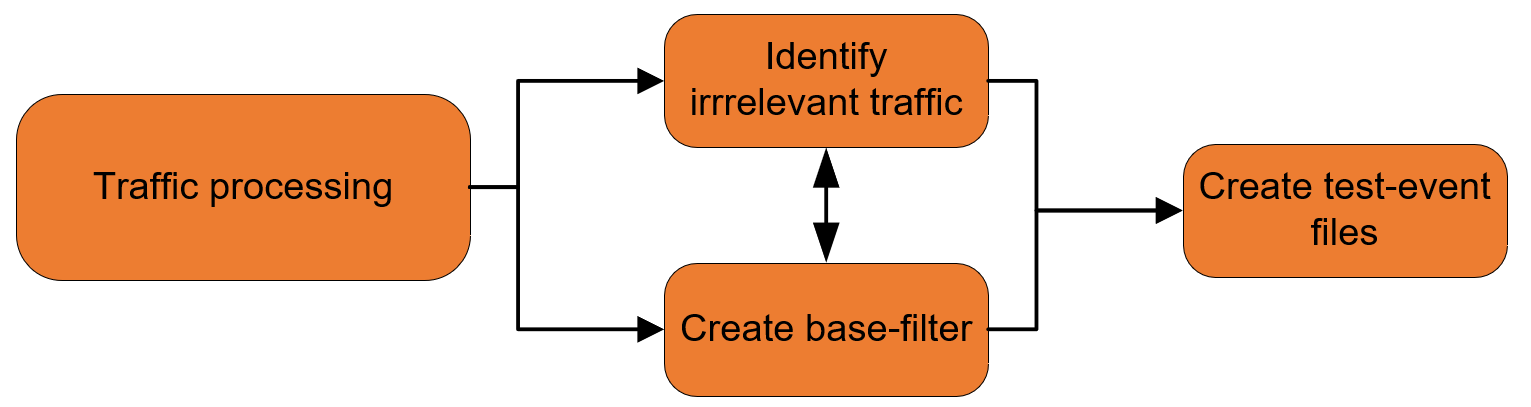
\includegraphics[width=\textwidth]{figures/TrafficProcessingProcess.png}
    \caption{Traffic filtering processing}
    \label{fig:TrafficProcessingProcess}
\end{figure}

The \textit{Standby traffic} capture is used to identify traffic patterns and protocols that are irrelevant to the event triggering conducted in this project. Since there was no interaction with the Irobot Roomba during the capturing period, all the identified traffic patterns and protocols are irrelevant for the actual event objectives. 

The capturing files are imported and opened in Wireshark and analyzed with the use of \textbf{Protocol hierarchy tools}. this tools presents the different protocols and their distribution within the capturing files. An example of this analysis is shown in Figure \ref{fig:wiresharkprotocolstatistictools}. Traffic from each of the identified protocols are analysed and irrelevant traffic observed is excluded by adding logical expressions to the baseline filter in Wireshark. Resulting in a complete baseline filter excluding all irrelevant traffic identified. 

\begin{figure}[H]
    \centering
    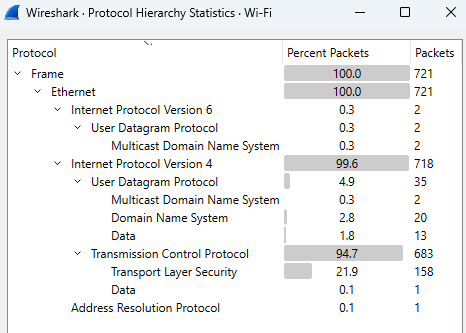
\includegraphics[width=0.8\textwidth]{figures/wireshark_protocol_hirarcy.png}
    \caption{Wireshark protocol hierarchy tool}
    \label{fig:wiresharkprotocolstatistictools}
\end{figure}

The basefilter is applied to the event capturing files and in addition a Wireshark time filter is added to only display traffic generated during an ongoing event, creating one capture file per event. The Wireshark filter syntax is found in \cite{wireshark} and the time filter syntax is presented below. 

\begin{itemize}
    \item \textbf{(frame.len >= "Year Month day, start-time") \&\& (frame.len <= "Year Month day, end-time")}
\end{itemize}



\section{Traffic Analysis}

The traffic analysis workflow is presented in Figure \ref{fig:TrafficAnalysisProcess}, and includes three subprocesses \textit{protocol and event relation, Traffic sequence identification} and \textit{Overall event characteristics}. Results from all these subprocesses were used to create event signatures. These signatures are implemented into python detection algorithms to evaluate the success rate of the signature detection. All events are analyzed with the same process described below.  

\begin{figure}[H]
    \centering
    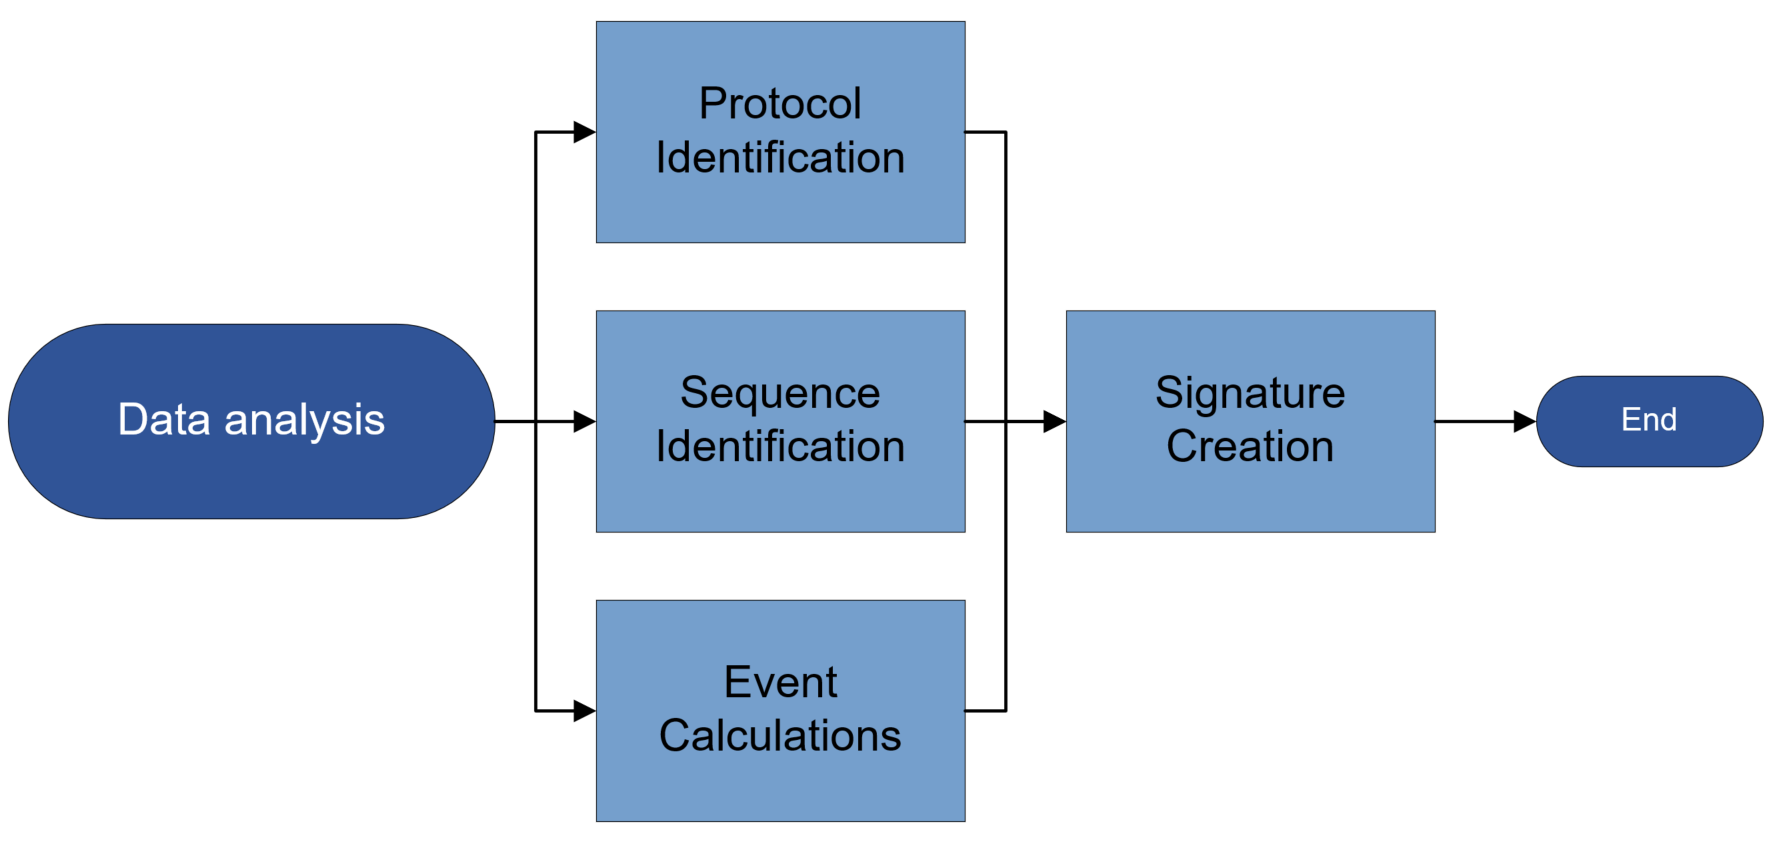
\includegraphics[width=\textwidth]{figures/TrafficAnalysisProcess.png}
    \caption{Traffic Analysis Process}
    \label{fig:TrafficAnalysisProcess}
\end{figure}

\textit{Protocol and event relation} are analyzed with \textbf{Protocol hierarchy tools} and the identified protocol and their attributes are collected. If specific protocols occur within the majority of the event files it could be used as a identification signature.

Traffic sequence analysis used same attributes as Trimananda et al.  \cite{pingpong_trimananda2020packet}, without the proposed machine learning algorithm. Packet length sequences were extracted with the use of a python script using a Pyshark library, and analyzed manually. This analysis also includes the sequence of protocols, enabling signatures based on more than just packet lengths as attributes. Traffic flow directions were also taken in to account during this process. This included the traffic flows listed below. 

\begin{itemize}
    \item Traffic flow with Irobot Roomba as source address.
    \item Traffic flow with Irobot Roomba as destination address.
    \item Traffic flow both directions.
\end{itemize}

\textit{Overall characteristics} of each event file were analyzed, and used to determine if the number of 20 events were sufficient. Extracted information about \textit{number of packets, total bytes sent} and \textit{protocols} were used in this process. Standard deviation of this data indicated the consistency of each event objective. 

Results of the three subprocesses were used to propose an event signature. Attributes in the different signatures were implemented as search conditions in a python function. A separate function was created for each event signature, returning a confident variable to the main function. This enables the detection algorithm to add new signatures to increase the detection confidence of an event. All these functions followed the same logical flow as presented in Figure \ref{fig:Sudo_code_signature_function}

\begin{figure}[H]
    \centering
    \caption{Pseudo code for signature detection function}
    \label{fig:Sudo_code_signature_function}
    \begin{lstlisting}[numbers=left]
     def Identify_event(event_file, event_confidence_variable):
         event_signature = ['signature']
         if event_signature is in eventfile:
             event_confident_variabel =+ level_of_confidece
         else
             None
         return event_confidence_variabel
    \end{lstlisting}
\end{figure}

\section{Signature Evaluation}
All signature functions were integrated in a main python script. This script imports selected pcap files and run through all the signature functions. True positive and False positive detection increases the confident variable for each event. A comparison of the confidence variables is executed at the end, to determine which event is most likely to have been triggered. The main function follows the logic presented in Figure \ref{fig:Sudo_code_event_detection_alg}. If a signature is identified in the majority of other events it can not be used to unlikely identify an event and will be rejected by this project. 

\begin{figure}[H]
    \centering
    \caption{Pseudo code event detection algorithm}
    \label{fig:Sudo_code_event_detection_alg}
    \begin{lstlisting}[numbers=left]
         Main()
              #import event pcap file
              Capture = import(Event_file_x)
              #run detection functions, and create confidence variables
              #eventX_confident_variable = eX_cv  
              e1_cv = identify_event1(Capture, event1_confidence_variable)
              e2_cv = identify_event2(Capture, event1_confidence_variable)
              e3_cv = identify_event3(Capture, event1_confidence_variable)
              e4_cv = identify_event4(Capture, event1_confidence_variable)
              e5_cv = identify_event5(Capture, event1_confidence_variable)
              e6_cv = identify_event6(Capture, event1_confidence_variable)
              #compare event_confident_variables highest is event
              confident_variables = [list of all variables]
              for event in range(1,6)
                   if confident_variabels[event] is larger than last number
                       largest = confident_variabels[event]  
    \end{lstlisting}
\end{figure}

Capture analysis is conducted on the LAN traffic due to time constrains within the project. To determine if the same method and type of signatures can be used to identify events in WLAN, a comparison is done between corresponding LAN and WLAN events. If the level of encryption is different for LAN and WLAN it is not possible to identify the same protocol distribution, and other signatures needs to be utilized. Packet length sequences is visible in all levels of network communication and differences are determined of included header lengths. A comparison is conducted to determine if the same sequences are present and if observed, the same method and type of filters can be used. 

